\chapter{Statistical phylogeography: Admixture graphs and {\tt sparg}}

Pickrell and Pritchard~\cite{Pickrell-Pritchard-2012} described the
most widely used approach to estimating admixture graphs. It is
implemented in {\tt TreeMix}.\index{TreeMix} At about the same time
Patterson et al.~\cite{Patterson-etal-2012} described a related method
at about the same time. I'm going to focus on the {\tt TreeMix}
approach because I am more comfortable with the underlying
model.\footnote{If you're curious about why I'm more comfortable with
  the Pickrell and Pritchard approach, feel free to ask.}
Unfortunately, if you want to use {\tt TreeMix}, you'll have to be comfortable
with compiling C++ programs from source~(or find a friend who can help
you or who can share a copy).\footnote{The most recent version of the
  {\tt TreeMix} manual notes that ``TreeMix should run on any Unix or
  Unix-like (e.g., Linux or Mac OS X) system. It may be more difficult
  to get it compiled under Windows. Notice that regardless of
  operating system, you'll also need to install the GNU Scientific
  Library and the Boost Graph Library.''}

The basic idea between {\tt Treemix} is not too complicated, although
it would be a stretch to say that it's simple. We start by assuming
that the allele frequencies are changing as a result of genetic
drift. Results going back to Kimura~\cite{Kimura-1955} tell us that
the variance in allele frequency is
\[
  \mbox{Var}(p_t) = p_o(1-p_0)\left(1 - e^{-t/2N_e}\right) \quad ,
\]
where $p_t$ is the allele frequency in the population at time $t$,
$p_o$ is the initial allele frequency, $t$ is the number of
generations, and $N_e$ is the effective population size. So long as
the effective population size is large enough that allele frequency
changes are relatively small from generation to generation and so long
as $p_o$ is not ``too close'' to 0 or 1, then we can approximate the
probability distribution of allele frequencies at time $t$ with a
normal distribution:
\[
  \mbox{P}(p_t|p_o,t,N_e) \sim \mbox{N}\left(p_o,
    p_o(1-p_o)\left(\frac{t}{2N_e}\right)\right) \quad .
\]
Now suppose we have a series of four populations related like those
shown in Figure~\ref{fig:treemix-no-migration}. As you can see, this
example shows populations that have a simple tree-like
relationship. Here's where the fun starts.

\begin{figure}
  \begin{center}
    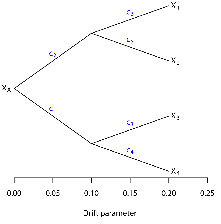
\includegraphics[width=12cm]{treemix-no-migration.eps}
  \end{center}
  \caption{A purely tree-like relationship among four hypothetical
    populations. The allele frequencies in each population are
    represented by $X_i$. The drift parameter on the $x$-axis is $t/2N_e$,
    i.e., it's measuring time from the root of the tree to the tips in
    units of $1/2N_e$. A part of a figure in~\cite{Pickrell-Pritchard-2012}.}\label{fig:treemix-no-migration}
\end{figure}

It's a well known fact~\cite{CavalliSforza-Edwards-1967} that the
variance in allele frequencies ($X_i$ in the figure) are simply
\begin{eqnarray*}
  \mbox{Var}(X_1) &=& (c_2 + c_6)X_A(1-X_A) \\
  \mbox{Var}(X_2) &=& (c_2 + c_5)X_A(1-X_A) \\
  \mbox{Var}(X_3) &=& (c_1 + c_3)X_A(1-X_A) \\
  \mbox{Var}(X_4) &=& (c_1 + c_4)X_A(1-X_A) \quad ,
\end{eqnarray*}
where $c_i = \frac{t_i}{2N_e^{(i)}}$, $t_i$ is the time associated
with branch $i$ and $N_e^{(i)}$ is the effective size of the
population associated with branch $i$. It's obvious from looking at
the tree that populations 1 and 2 have been evolving independently
from populations 3 and 4 from the start, while 1 and 2 have been
evolving independently of one another for a shorter period of time. As
a result, we expect allele frequencies in pouplations 1 and 2 to be
more similar than those in populations 3 and 4. In fact, Pickrell and
Pritchard point out that we can write the various covariances down
pretty simply too:
\begin{eqnarray*}
  \mbox{Cov}(X_1,X_2) &=& c_2X_A(1-X_A) \\
  \mbox{Cov}(X_1,X_3) &=& 0 \\
  \mbox{Cov}(X_1,X_4) &=& 0 \\
  \mbox{Cov}(X_2,X_3) &=& 0 \\
  \mbox{Cov}(X_2,X_4) &=& 0 \\
  \mbox{Cov}(X_3,X_4) &=& c_1X_A(1-X_A) \quad .
\end{eqnarray*}
As a result, we can write down a multivariate probability distribution
that describes all of the allele frequencies simultaneously, given the
same caveats as above about the normal distribution.
\[
  \mbox{P}(\bf p_t|\bf p_0, \bf t, \bf N_e) \sim \mbox{MVN}(\bf p_0,
  \bf \Sigma) \quad ,
\]
where boldface refers to vectors, MVN refers to the multivariate
normal distribution, and $\bf Sigma$ is the covariance matrix of
allele frequencies. Since we can write down that probability
distribution, you can probably imagine that it's possible to estimate
the likelihood of our data given a particular tree. To get a maximum
likelihood estimate of how our populations are related, assuming
there's no migration, we simply have to compare the likelihoods across
all possible trees and choose the one that's most likely.\footnote{If
  you know anything about estimating phylogenies, you know there is
  tremendous complexity buried in that ``simply have to compare.''
  Also notice that if we can get a maximum likelihood estimate, we can
  also get a full Bayesian posterior ``simply'' by providing the
  appropriate priors.}

Now suppose we allow migration from one of our populations into
another. The simple example Pickrell and Pritchard
provide~(Figure~\ref{fig:treemix-figure} shows a single migration from
the lineage leading to population 2 into population 3, labeling the
source population as $Y$ and the destination population as $Z$. As you
can see in Panel D of the figure, the migration event changes the
structure of the covariance matrix. Since all the migration event does
is to change the covariance matrix, we can once again explore
parameter space and find the network that maximizes the
likelihood. When we do so, not only do we have estimates for
population relationships and effective population sizes but also for
the timing and direction of migration events. Estimating admixture is,
however, even more challenging than estimating a population
phylogeny. The number of alternative configurations explodes rapidly
with more than 4-5 populations, making heuristic searches
necessary. Molloy et al.~\cite{Molloy-etal-2021} recently described a
new approach that builds on {\tt TreeMix} and seems to avoid getting
stuck in a local optimum. Since the basic approach is the same and
this isn't a course in computational biology, we won't discuss it
further, but you should investigate it if you use admixture graphs in
any of your work.

\begin{figure}
  \begin{center}
    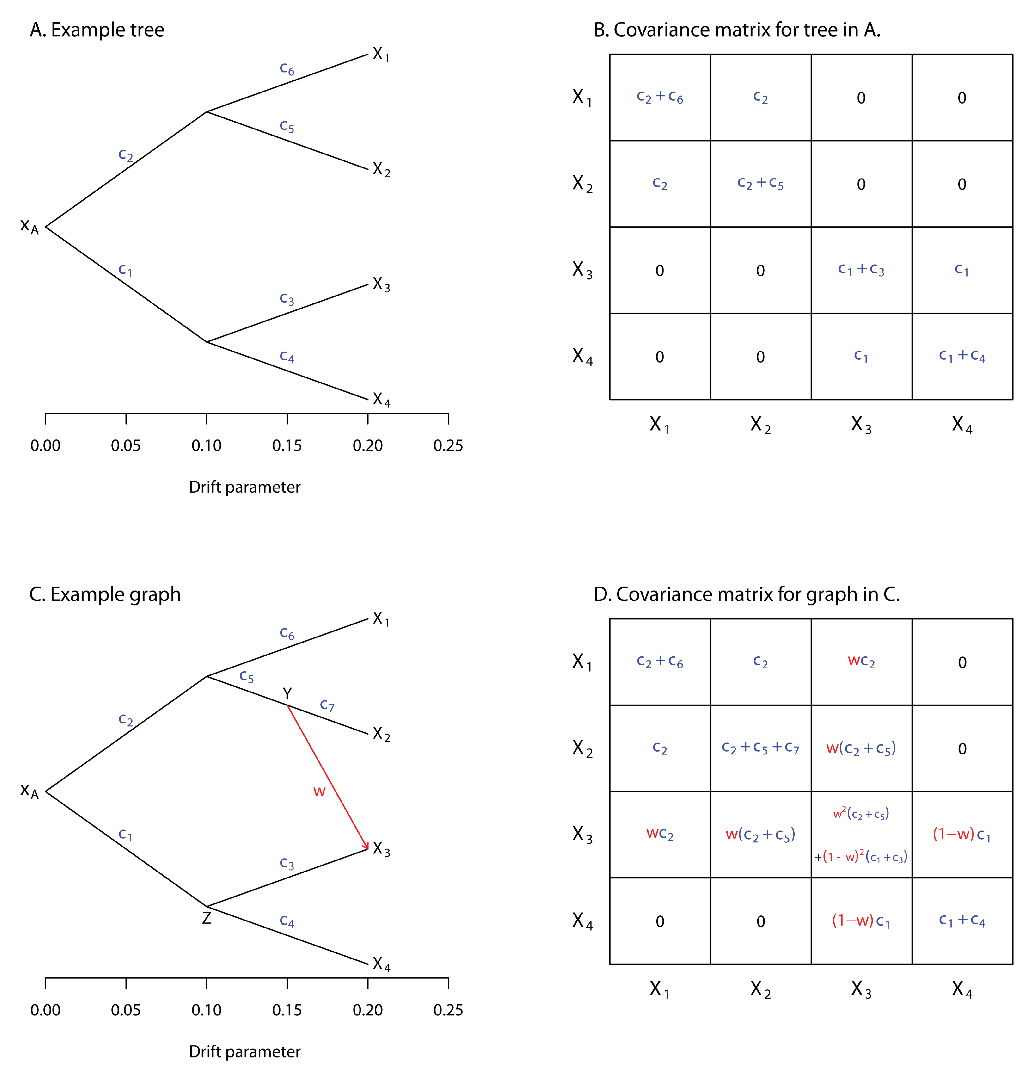
\includegraphics[width=14cm]{treemix-figure.eps}
  \end{center}
  \caption{Illustrating the covariance matrices of admixed and
    unadmixed populations. From \cite{Pickrell-Pritchard-2012}.}\label{fig:treemix-figure}
\end{figure}

\section*{Estimating dispersal and ancestral
  geography}\index{ancestral geography}\index{sparg@{\tt sparg}}

As you can see, admixture graphs provide a very flexible approach to
understanding the history of populations. But they do have one
significant limitation. We have to know ahead of time which
indivdiuals belong in which populations, just as we did with
$F$-statistics,\index{F-statistics@$F$-statistics} and just as with
{\tt STRUCTURE} gave us a way to look at population structure without
pre-assigning individuals to populations, there's a way of looking at
ancestry that uses individuals rather than pre-defined
populations~\cite{Osmond-Coop-2021}. As with admixture graphs, the
mathematics lying behind the approach gets pretty hairy, but the basic
idea is pretty simple~(Figure~\ref{fig:sparg-overview}).

\begin{figure}
  \begin{center}
    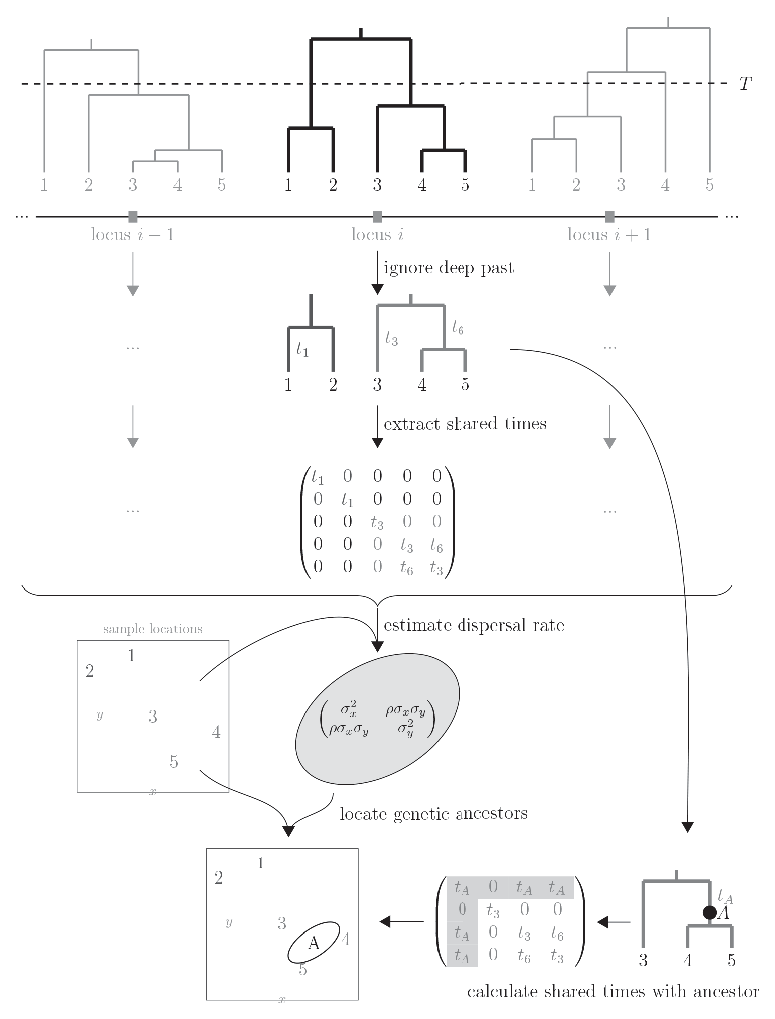
\includegraphics[width=14cm]{sparg-overview.eps}
  \end{center}
  \caption{Conceptual overview of the process for estimating the
    spatial position of ancestors
    (from~\cite{Osmond-Coop-2021}).}\label{fig:sparg-overview} 
\end{figure}

\begin{itemize}

  \item At any position along a genome, we can construct a
    phylogeneitc tree showing the genealogical relationship among all
    chromosomes in the sample at that location.\footnote{Notice that I
      wrote ``chromosomes'', not individuals, because the different
      allele copies within an individual may have different
      genealogical histories.} 

  \item Individuals disperse randomly through space with the distance
    of an offspring from its mother given by a bivariate normal
    distribution with a mean of 0 and a covariance matrix
    $\bf\Sigma$. In any real sample, glacial migrations,
    barriers to dispersal, or the opening of new habitat will cause
    some aspects of the dispersal history not to be well approximated
    by this model of Brownian motion, so we only use parts of the tree
    from the first step that are more recent than these events to
    estimate dispersal parameters.\footnote{Notice that while this
      approach means that the Brownian motion model for disperal is a
      better fit to the data, it also means that we can't use this
      approach to study events that involve ancient dispersal, like
      early modern human movemeents out of Africa.}

  \item Given the estimates of time to a common ancestor between two
    individuals, the spatial location of those individuals, and the
    dispersal rate, we can estimate the spatial location of the
    ancestor. 

\end{itemize}

This method implicitly assumes that differences are selectively
neutral.\footnote{Remember: This doesn't mean that there aren't any
  fitness differences, only that the product of the selection
  coefficient associated with any of those differences and the
  population size is less than one, implying that the evolutionary
  dynamics are rougly similar to those of a purely neutral locus.}
Although we could try this approach with data from only one locus, the
results are unlikely to be informative for two reasons. First, there
is a lot of uncertainty associated with our estimate of phylogenetic
relationships at one locus. Second, because the coalescent history of
unlinked loci will differ even though the effective population size
and the patterns of migration that affect different loci are the
same. But since the patterns of migration {\it are\/} the same across
different loci and since the effective population size {\it is\/} the
same across loci, we can combine information across loci to get better
estimates of the dispersal rates. Since we estimate the location of
ancestors at every locus, we end up with a distribution of ancestral
locations rather than a single estimate. Osmond and Coop also point
out that we can define different ``epochs'' in which to estimate
dispersal rates and ancestors. This allows the dispersal rate to vary
over time. All of this is available in a Python package, {\tt sparg},
which should run on any platfrom with
phython3~(\url{https://github.com/mmosmond/sparg}).

\subsection*{An example from {\it Arabidopsis}}\index{Arabidopsis@{\it Arabidopsis thaliana}} 

Plant geneticists have studied {\it Arabidopsis thaliana\/}
extensively. Alonso-Blanco et al.~\cite{AlonsoBlanco-etal-2016}
reported results derived from sequencing 1135 different wild
accessions derived from Eurasia and North Africa. Osmond and Coop used
{\tt sparg} to explore historical patterns of disperal and the
geographical location of ancestors using this data set. They first
estimated dispersal rates in both a one-epoch model and in multi-epoch
models. As you can see in Figure~\ref{fig:arabidopsis-epochs}), the
estimates of dispersal rates are very similar across all of the
loci. In addition, the per-generation rate of east-west dispersal
($\sigma^2_{long}$) is about 10 times higher than north-sourth
dispersal ($\sigma^2_{lat}$), and the correlation between the two
rates ($\rho$) is relatively small. Comparison among the scenarios
suggests that the 4-epoch model is the best fit to the data,
suggesting that the rate of dispersal in the last 10 generations is
substantially greater than it was earlier and that dispersal between
10 and 1000 generations ago is greater than it was more than 1000
generations ago.

\begin{figure}
  \begin{center}
    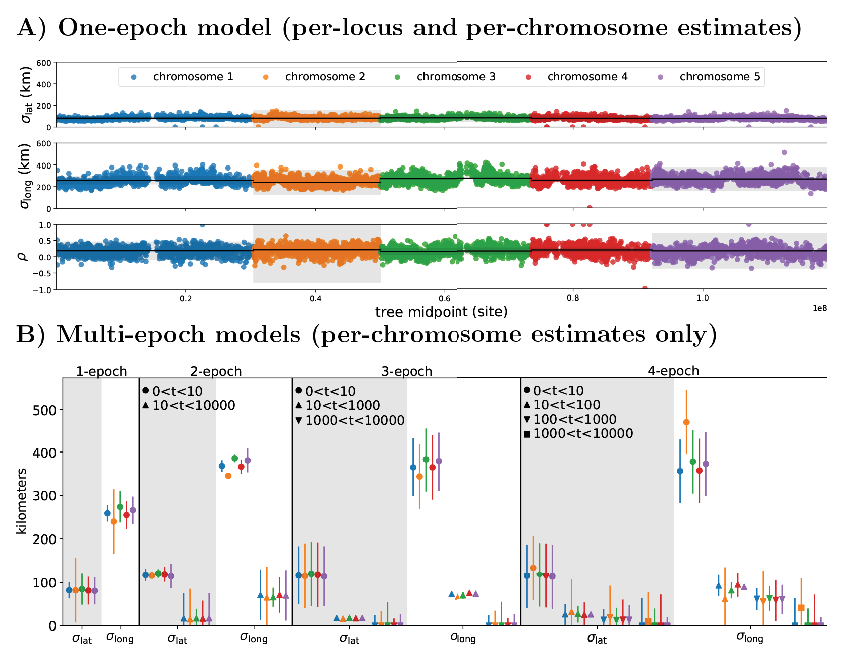
\includegraphics[width=14cm]{arabidopsis-epochs.eps}
  \end{center}
  \caption{Estimates of dispersal rates in {\it Arabidopsis
      thaliana\/} in both one-epoch (panel A) and multi-epoch (panel
    B) models (from~\cite{Osmond-Coop-2021}).}\label{fig:arabidopsis-epochs}
\end{figure}

Now that we have a good idea {\it when\/} dispersal happened, let's
see {\it where\/} it happened. As you can see in
Figure~\ref{fig:arabidopsis-dispersal}, much of the estimated
dispersal over the last 10-100 generations didn't move individuals
very far. In addition, it's a little hard to see, but if you zoom in
on the figure and focus on the purple colors, you'll notice that most
of the lines leading from the dots~(current locations) point towards
the center of Europe. This pattern is particularly clear in for the
100-generation ago ancestral location of samples from
Scandinavia. There are, however, a few individuals that moved very
long distances. Individual 9627, for example, seems to have an ancestor 10
generations ago that was more than 3000km to the east of its current
location, and its ancestor seems to have been more than 4000km to the
east 100 generations ago.

\begin{figure}
  \begin{center}
    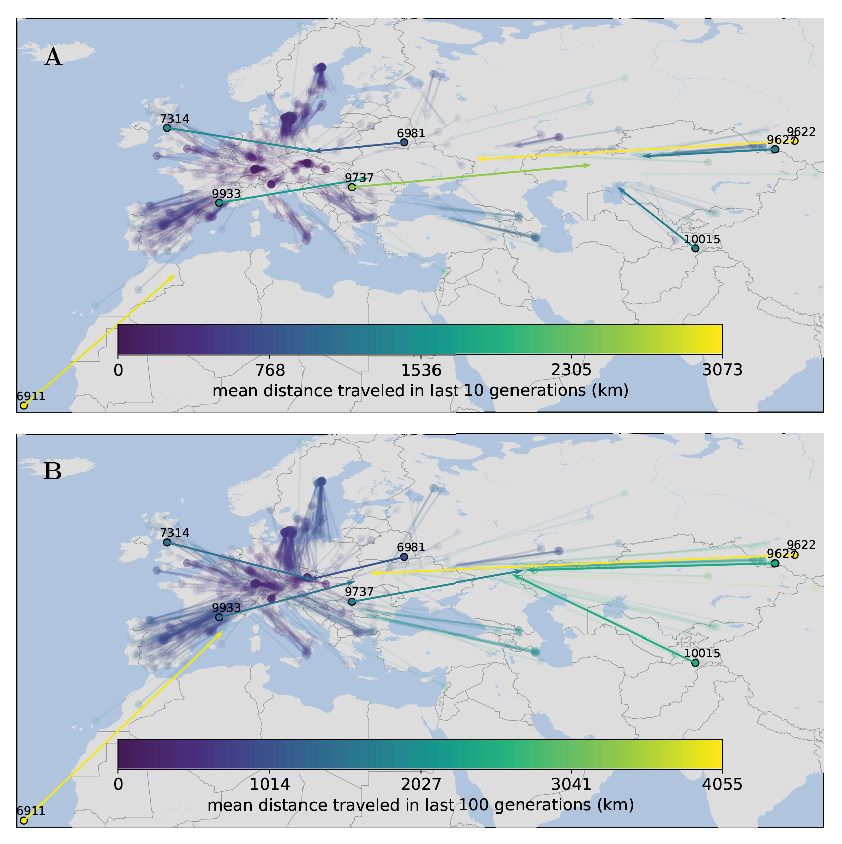
\includegraphics[width=14cm]{arabidopsis-dispersal.eps}
  \end{center}
  \caption{Estimates of the ancestral location of {\it Arabidopsis
      thaliana\/} accessions 10 and 100 generations ago
    (from~\cite{Osmond-Coop-2021}).}\label{fig:arabidopsis-dispersal}
\end{figure}

